% This version uses the latex2e styles, not the very ancient 2.09 stuff.
\documentclass{sig-alternate-10pt}
\usepackage{endnotes,url}
%\usepackage{sig-alternate-10pt,endnotes}
\usepackage{epsfig}
\usepackage{amssymb}
\usepackage{amsmath}
\usepackage{algorithm}
\usepackage{algorithmic}
\usepackage{amsfonts}
\usepackage{graphicx}
\usepackage{verbatim}
% Replaced by subfig package
% \usepackage{subfigure}
\usepackage{subfig}
\usepackage{epstopdf}
\usepackage{cite}
\usepackage{array}
\usepackage{multirow}
\usepackage{listings}


%\pdfpagewidth 8.5in
%\pdfpageheight 11in
%\baselineskip=12.5pt
%\setlength{\pdfpagewidth}{8.5in}
%\setlength{\pdfpageheight}{11in}
%\usepackage{pdfdraftcopy}

% To import classical math notation used

% Mathematical LaTeX formatting shortcuts
\newcommand{\midwor}[1]{\;\textnormal{ #1 }\;} % text in math mode
\newcommand{\ds}{\displaystyle} % shorcut to toggle display
	% All formula should punctuation as they are part of the text.
\newcommand{\vf}{\,,\,} % a comma with space
\newcommand{\ff}{\,.} % a dot 
	% The following command allows to write quickly sets { }   
\newcommand{\lset}{\left\{\left.\;}
\newcommand{\midset}{\;\right|\;\left.}
\newcommand{\dimset}{\right.\;\left|\;}
\newcommand{\rset}{\;\right.\right\}}
\newcommand{\jset}{\right.\right.\\ & \left.\left.}

% Number sets and usual operations
\newcommand{\Real}{\mathbb{R}} % real numbers
\newcommand{\RelInt}{\mathbb{Z}} % relative integer numbers
\newcommand{\NatInt}{\mathbb{N}} % natural integer numbers
\newcommand{\Compl}{\mathbb{C}} % complex numbers
\newcommand{\valent}[1]{\left\lfloor #1 \right\rfloor} % integer value
\newcommand{\valentsup}[1]{\left\lceil #1 \right\rceil} % integer value + 1
\newcommand{\eps}{\varepsilon} % very small real number
\newcommand{\argmin}{\textrm{argmin}} %argument of the minimum
\newcommand{\pospar}[1]{\left( #1 \right)^+} % positive part

% Probability notation
\newcommand{\proba}{\mathbb{P}} % Probability
\newcommand{\probaof}[1]{\mathbb{P}\left.\left[#1\right.\right]} % Probability of an event
\newcommand{\cond}{\right|\left.} % Condition on an event 
\newcommand{\expec}[1]{\mathbb{E}\left[#1\right]} % Expectation 
\newcommand{\vari}[1]{\textrm{V}\left[#1\right]} % Variance 
\newcommand{\Lun}{\mathbb{L}^{1}} % Space of integrable function
\newcommand{\as}{\;\textrm{a.s.}\;}
\newcommand{\ind}[1]{\mathbb{I}_{\{#1\}}} % Indicator
\newcommand{\tribF}{\mathcal{F}} % sigma-algebra

% Constants
\newcommand{\cst}{\textrm{\texttt{cst}}}

% Advanced probability 
\newcommand{\comp}{\circ} % composition of function
\newcommand{\shi}{\theta} % ergodic shift
\newcommand{\lstoc}{\displaystyle \leq_{\textrm{st}}} % Stochastic Order
\newcommand{\Ppalmof}[1]{\mathbb{P}^{0}_{#1}}
\newcommand{\Pofpalmof}[2]{\mathbb{P}^{0}_{#1}\left[#2\right]}
\newcommand{\expPalm}[1]{\mathbb{E}^{0}[#1]} % Palm Expectation
\newcommand{\expPalmof}[2]{\mathbb{E}^{0}_{#1}[#2]} % Palm Expectation w.r.t. point process f 

% (max,+) algebra
\newcommand{\Rmax}{\mathbb{R}_{\max}}
\newcommand{\ninf}{\varepsilon}
\newcommand{\matninf}{\textrm{\Large{$\ninf$}}}
\newcommand{\zer}{e}
\newcommand{\veczer}{\textrm{\Large{e}}}
\newcommand{\bigmax}{\bigvee}
\newcommand{\matId}{{\mathbb{I}}}
%\newcommand{\norm}[1]{\| #1 \|}
\newcommand{\linf}[1]{\left|\left| #1 \right|\right|}

% Matrices
\newcommand{\matA}{\mathbb{A}}
\newcommand{\matB}{\mathbb{B}}
\newcommand{\matC}{\mathbb{C}}
\newcommand{\matP}{\mathbb{P}}
\newcommand{\matQ}{\mathbb{Q}}

% Used for set
\newcommand{\setI}{\mathcal{I}}
\newcommand{\setJ}{\mathcal{J}}
\newcommand{\setK}{\mathcal{K}}
\newcommand{\setL}{\mathcal{L}}

% Users and Buckets
\newcommand{\setU}{\mathcal{U}}
\newcommand{\setC}{\mathcal{C}}

\newcommand{\setA}{\mathcal{A}}
\newcommand{\setW}{\mathcal{W}}

% Used for set
\newcommand{\setN}{\mathcal{N}}
\newcommand{\setS}{\mathcal{S}}


\newenvironment{disarray}%
 {\everymath{\displaystyle\everymath{}}\array}%
 {\endarray}

 \newcommand{\pdi}[1]{\frac{\partial #1}{\partial x_i}}
 \newcommand{\pdj}[1]{\frac{\partial #1}{\partial x_j}}

% Package for date and time presentation
\usepackage{datetime}
\newcommand{\datation}{\today, \xxivtime}

\def\full{0}        % set 1 for a full tech report version
                    % set 0 for submission version
\def\shownotes{1}   % set 1 for version with author notes
                    % set 0 for no notes
\def\anon{0}        % set 1 to anonymize
                    % set 0 for acks and author names

%%%%%%%  Author Notes %%%%%%%
%
\ifnum\shownotes=1
\newcommand{\authnote}[2]{{ $\ll$\textsf{\footnotesize #1 notes: #2}$\gg$}}
\else
\newcommand{\authnote}[2]{}
\fi
\newcommand{\Ynote}[1]{{\authnote{Yan}{#1}}}
\newcommand{\Anote}[1]{{\authnote{Andrius}{#1}}}
\newcommand{\Nnote}[1]{{\authnote{Narseo}{#1}}}
\newcommand{\Vnote}[1]{{\authnote{Vijay}{#1}}}
\newcommand{\Dnote}[1]{{\authnote{Dina}{#1}}}

%%%%%%%%%%%%%%%%%%%%%%%%%%%%%%%%%

\newcommand{\namedref}[2]{#1~\ref{#2}}
\newcommand{\tableref}[1]{\namedref{Table}{#1}}
\newcommand{\sectionref}[1]{\namedref{Section}{#1}}
\newcommand{\appendixref}[1]{\namedref{Appendix}{#1}}
\newcommand{\theoremref}[1]{\namedref{Theorem}{#1}}
\newcommand{\remarkref}[1]{\namedref{Remark}{#1}}
\newcommand{\definitionref}[1]{\namedref{Definition}{#1}}
\newcommand{\figureref}[1]{\namedref{Figure}{#1}}
\newcommand{\lemmaref}[1]{\namedref{Lemma}{#1}}
\newcommand{\claimref}[1]{\namedref{Claim}{#1}}
\newcommand{\propositionref}[1]{\namedref{Proposition}{#1}}
\newcommand{\constructionref}[1]{\namedref{Construction}{#1}}
\newcommand{\corollaryref}[1]{\namedref{Corollary}{#1}}
\newcommand{\equationref}[1]{\namedref{Equation}{#1}}
%
\newtheorem{theorem}{Theorem}[section]
\newtheorem{definition}[theorem]{Definition}
\newtheorem{lemma}[theorem]{Lemma}
\newtheorem{claim}[theorem]{Claim}
\newtheorem{obs}[theorem]{Observation}
%


\providecommand{\vs}{vs. }
\providecommand{\ie}{\emph{i.e.,} }
\providecommand{\eg}{\emph{e.g.,} }
\providecommand{\cf}{\emph{cf.,} }
\providecommand{\resp}{\emph{resp.,} }
\providecommand{\etal}{\emph{et al.}}   %Removed trailing space here; usually want non-breaking space with following reference
\providecommand{\etc}{\emph{etc.}}      % No trailing space here either
\providecommand{\mypara}[1]{\smallskip\noindent\emph{#1} }
\providecommand{\myparab}[1]{\smallskip\noindent\textbf{#1} }
\providecommand{\myparasc}[1]{\smallskip\noindent\textsc{#1} }
\providecommand{\para}{\smallskip\noindent}

\newtheorem{axiom}{{\bf  Axiom}}
\newtheorem{defin}{{\bf  Definition}}
\newtheorem{proposition}{Proposition}

\usepackage{enumitem}
\setlist{nolistsep}

%Model parameters

\usepackage[breaklinks=true]{hyperref}
\frenchspacing
\begin{document}

%don't want date printed
\date{}


%make title bold and 14 pt font (Latex default is non-bold, 16 pt)
\title{Demo: PhoneLets -- offloading the phone off your phone for energy, cost and network load optimization}
\ifnum\anon=1
\author{[Paper: \#XXX]}% \hspace{0.2cm} \ampmtime ]}
\else
\numberofauthors{2}
\author{
\alignauthor Andrius Aucinas\\
\affaddr{University of Cambridge} 
\and
\alignauthor Jon Crowcroft\\
\affaddr{University of Cambridge}
}
\fi
%for single author (just remove % characters)

    
% end author
\maketitle
% Use the following at camera-ready time to suppress page numbers.
% Comment it out when you first submit the paper for review.
%\thispagestyle{empty}
\begin{abstract}
This demo presents how phone functionality can be offloaded from a smartphone over wireless link to a \emph{PhoneLet} by sharing one SIM card across multiple devices. This can lead to significant cost and network load reductions by reducing the number of simultaneously connected mobile clients. Furthermore, it can bring significant energy reductions for the mobile user when connected to a powered \emph{PhoneLet}. It absorbs the energy cost of inefficient mobile applications' communication patterns, instead providing connectivity for the user over a WiFi link.
\end{abstract} 

\section{What PhoneLets are}
\label{section:intro}

A modern smartphone has more in common with a computer than a phone, and connectivity to the Internet and surrounding devices (the \emph{Internet of Things}) is tipping the balance even further. Importance of cellular networks, however, remains as they provide almost ubiquitous Internet connectivity around the world. Cellular connectivity has its own problems. This demo shows how PhoneLets allow one SIM (Subscriber Identity Module) to be shared between nearby devices. This addresses the following problems with cellular connectivity:

Firstly, connectivity is relatively expensive for users~\cite{Anonymous:2013ut}, typically requiring a separate subscription for each device connected to the cellular network, e.g. smartphone and tablet as well as broadband connectivity at home and at work. Using PhoneLets to share a single SIM across devices solves this issue.

Secondly, the increasing number of connected, periodically communicating clients increases infrastructure costs and also increases cellular network load, in extreme cases causing \emph{signaling storms}~\cite{Yang:wh} that can bring down an entire network. PhoneLets reduces the number of simultaneously connected clients by sharing the same cellular link across multiple clients.

Finally, energy consumption of always connected clients is high compared to short-range radio technologies. Sharing a cellular link also helps reduce it for mobile devices.

\emph{PhoneLets} enable phone offloading by exploiting remote SIM functionality of existing hardware. A cellular module exchange commands with a SIM/UICC module over a wireless communication link rather than direct, physical connection. Uses of such technology have included automotive as well as electronic currency~\cite{subramanian2003sim}. \emph{PhoneLets} infrastructure establishes and manages secure communication channels between participating entities and allows a device to connect to a cellular network without a physical SIM module being present.


\section{PhoneLets Design}

\begin{figure}
\centering
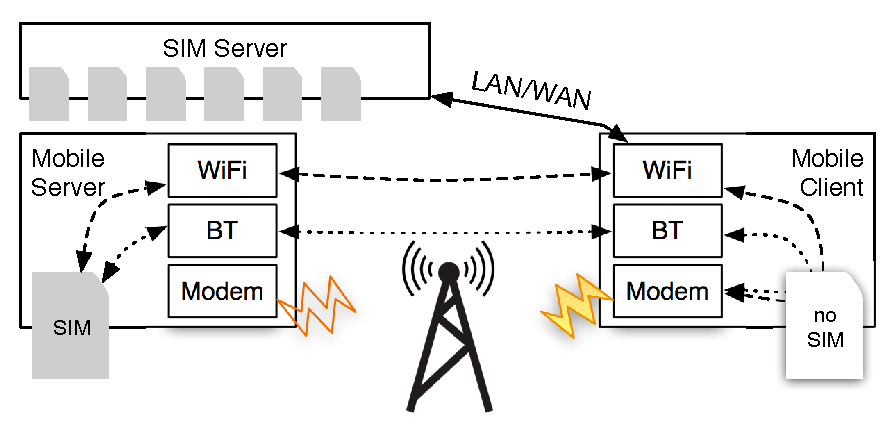
\includegraphics[width=0.9\columnwidth]{figs/arch}
\vspace{-3mm}
\caption{Architecture}
\label{fig:arch}
\vspace{-2mm}
\end{figure}

The overall concept and system architecture is shown in Fig.~\ref{fig:arch}. There are three types of entities: 1) mobile server, a mobile device which can share its SIM with other clients, 2) SIM server which may host and provide more sets of credentials over local or wide-area networks and 3) a mobile client which can use either of the methods.

Our design extends the standardized RSAP (Remote SIM Access Protocol) version by using a SIM server which is not capable of mobile connectivity itself and by using arbitrary communication links to access a remote SIM card (\emph{no SIM} in the mobile client). Our work for this demo focused primarily on the client and SIM server design, and we are using off-the-shelf hardware as the mobile server to demonstrate backwards-compatibility.

\begin{figure}[t!]
\centering
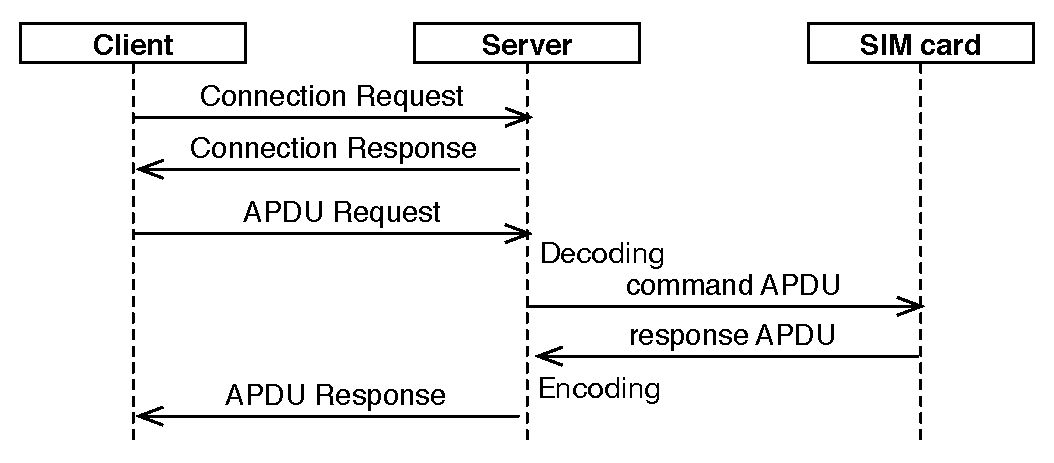
\includegraphics[width=0.9\columnwidth]{figs/sequence}
% \vspace{-2mm}
\caption{Communication sequence between client, server and remote SIM card}
\label{fig:sequence}
% \vspace{-4mm}
\end{figure}

The mobile Client can obtain network credentials from any server -- a user's mobile phone, a co-located or a remote SIM server -- as long as it can reach it. The key observation is that there are few operations that require access to the SIM card due to its interface speed (it would be infeasible to use it on the data path) and instead it is used to generate encryption keys. The generating keys, however, can never be accessed directly. Part of the network's security however comes from the network authenticating the subscriber for any major operation (e.g. placing or receiving calls, establishing PDP context). The cellular module therefore must always be able to access the remote card using standard Application Protocol Data Unit (APDU) messages (Fig.~\ref{fig:sequence}).

Importantly, we do not clone the SIM card and by design the system disables connectivity for one device before enabling it for another one to prevent multiple devices sharing the same credentials simultaneously. Only one device is connected to the cellular network and may share (\emph{tether}) the connectivity to other devices over another channel. One cellular module is also only capable of being registered with one network, enforcing a strict one-to-one mapping.

\subsection{Prototype}

\begin{figure}[t!]
\centering
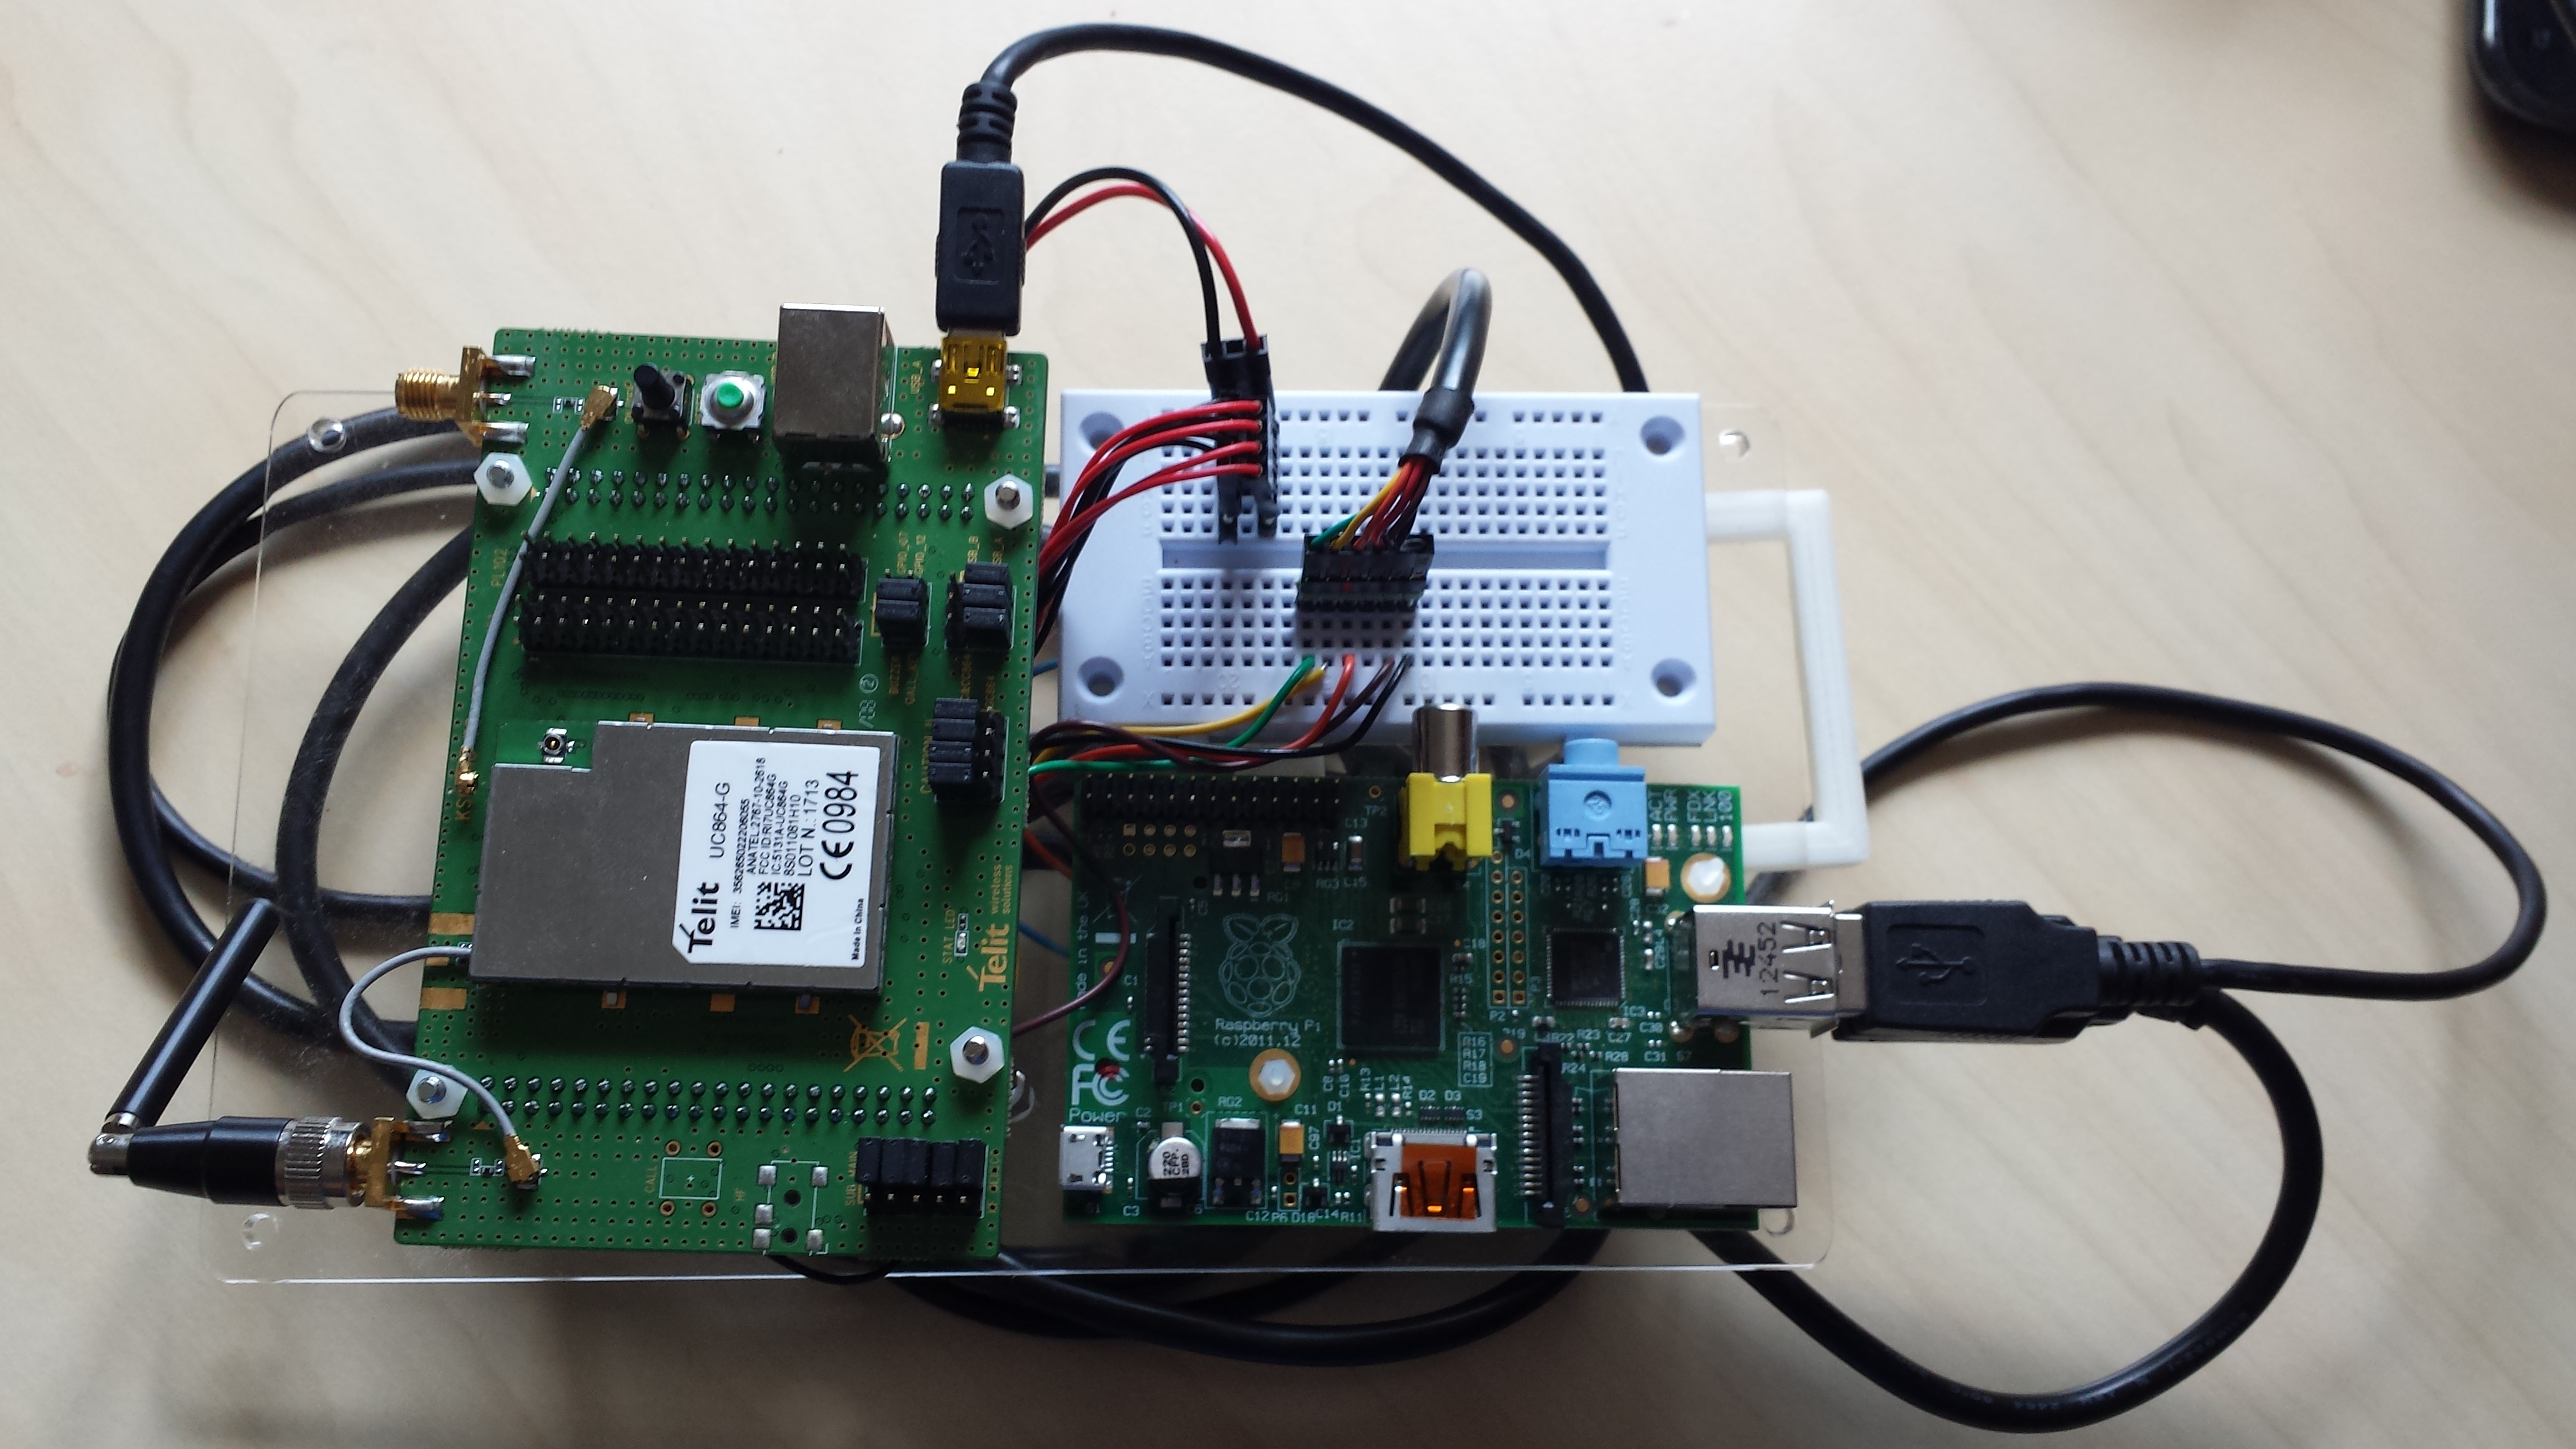
\includegraphics[width=0.9\columnwidth]{figs/client}
% \vspace{-2mm}
\caption{Client prototype}
\label{fig:client}
% \vspace{-3mm}
\end{figure}

Our demo mobile client (Fig.~\ref{fig:client}), the \emph{PhoneLet}, consists of a Telit UC864 cellular module connected to a raspberryPI as a controller, which also uses WiFi and BlueTooth dongles for local wireless connectivity. The controller runs a modified version of the Ofono open telephony stack and manages communication between the cellular module and multiple backends.

The two servers are an off-the-shelf Samsung Galaxy S4 and our custom server that only interfaces with SIM cards through a smartcard reader, also running on a raspberryPI. In our prototype, the server is connected to a WiFi AP to be reachable by the mobile client. We replace the BlueTooth communication channel with a more secure option - TCP link with certificate-based authentication of both client and server, and strong encryption for all data exchange. Once the client establishes a connection to either backend, it registers with the network and takes on the role of a phone.

\section{Energy saving opportunities}
\label{sec:energy}

Reduced mobile client energy consumption is an important motivation for \emph{PhoneLets}. We analyze energy consumption of the client in a few example scenarios using our early prototype. The \emph{PhoneLet} itself is not yet energy-optimized, i.e. the controlling RaspberryPI is not meant for mobile uses, so we focused on energy comparison of the mobile SIM server - a phone carried by the user from which we offload phone functionality.

\begin{table}[t]
{
\small
\begin{tabular}{| l | c |}
\hline
  \textbf{Use case}         & \textbf{Energy consumption (mA)}  \\ \hline
  Idle - airplane mode      & 5     \\ \hline
  Ifle - BlueTooth          & 6     \\ \hline
  Idle - WiFi               & 8     \\ \hline
  Idle - 3G                 & 10    \\ \hline
  Apps background - WiFi    & 27    \\ \hline
  BlueTooth SIM access      & 28    \\ \hline
  Apps background - 3G      & 40    \\ \hline
  WiFi tethering (idle)     & 80    \\ \hline
\end{tabular}
}
% \vspace{-2mm}
\caption{Energy consumption of an idle device with different radios enabled. (Apps background = Google apps and Facebook)}
\label{tab:energy}
% \vspace{-3mm}
\end{table}

Energy consumption of a Samsung Galaxy S4 was measured\footnote{Using Monsoon Power Monitor \url{http://www.msoon.com/LabEquipment/PowerMonitor/}} in a number of scenarios. The different values are presented in Table.~\ref{tab:energy}\footnote{Energy consumption provided as average current drawn because it is independent of current battery voltage}. 

The absolute values will vary with different devices and network configuration or conditions and application use, but the overall results remain. In particular, energy consumption of the different idle radios is similar, but cellular networks are significantly less efficient for current applications' network usage patterns~\cite{Aucinas:2013uk}. Therefore, replacing the cellular link with a WiFi one to another, powered device can bring significant savings - 32.5\% in our example case.

The default BlueTooth implementation of RSAP is not efficient enough - maintaining access alone consumes almost three times the amount of energy of an idle device connected to a 3G network. Instead, we have implemented SIM sharing over WiFi using our custom client and verified that the BlueTooth version is unnecessarily wasteful - once the PhoneLet has registered to the network, there is no communication with the SIM server for as long as the device is idle. For example, a phonecall is successfully received after 30 minutes of no activity. The current Android platform does not allow RSAP to run over WiFi, but based on our measurements we expect energy consumption of an optimized implementation to be very close to that of an idle WiFi channel - 3.5x less than BlueTooth.

Finally, we measured energy consumption of WiFi tethering. With just one idle client it is almost 3x higher than the BlueTooth case. RSAP is effectively an alternative to WiFi tethering when the mobile client provides connectivity to other devices. So similarly to above, we expect energy consumption of an optimized WiFi mobile client to be close to 10x less than WiFi tethering.

These are early results, but they point to a potential use-case where a powered \emph{PhoneLet} is registered to the network on behalf of a WiFi-connected client at a considerable energy benefit. Outside the scope of this demo, the benefit would be further improved when network access is shared across multiple such devices and SIM access load is balanced across them as the savings for each individual device would add up.

\section{Demo: wireless SIM sharing}

To demonstrate the working prototype of the system, we show our client \emph{PhoneLet} (Fig.~\ref{fig:client}), communicating with an off-the shelf mobile device or our SIM server to share their credentials for network registration in the following steps:

\begin{enumerate}
    \item Make a phone call to the mobile server (phone) and show that it is ringing
    \item Start sharing its SIM card with the client and show that the client is registered to the network with the same ID by making a phone call to it
    \item Start using SIM card in the SIM server over WiFi and show that the client is registered to the network with a different ID by making a call to the other number.
\end{enumerate}

In the three steps we show our prototype's ability to offload phone functionality from a phone - share subscriber credentials between multiple clients and select which one will be connected to the network.

\section{Discussion}

In addition to connectivity, \emph{PhoneLets} offers management of an individual's ID - the phone number. There have been multiple offerings with such function: multiple SIM cards associated with a number or VoIP-based solutions (\eg Google Voice), however they do not solve the problem of an increasing number of cellular clients and billing depends on service provider.

One cellular network in UK has offered a service to make phonecalls from tablets and laptops over WiFi to its users using a special app\footnote{O2 TU Go \url{http://www.o2.co.uk/apps/tu-go}} further blurring the line between mobile and the Internet. If WiFi Internet connectivity is available, the approach could help reduce energy consumption by disabling cellular radio.

Reprogrammable SIM cards~\cite{OFcom:2012tx} such as embedded SIM~\cite{Association:2013ub} have been proposed for provisioning in M2M communication. They maintain a physical secure element to store credentials, but provide mechanisms to manage them over the air. The architecture, allows operators to retain full control over the credentials, including when new ones can be installed or old ones removed, with necessarily centralized management and reduced flexibility on the client side.

Finally, questions that remain to be answered in future work include not only optimizations of the management and control protocols, but also the development of usage policies in multi-user environments and guaranteed isolation properties as well as adaptation of energy-aware routing protocols for distributed nodes.

\section{Summary}

Increasingly, smartphones are replicating computer use, with phone now a very secondary function to email, social media and entertainment. However mobile network connections remain expensive both financially and in terms of the energy they use. \emph{PhoneLets} is a system that allows a single mobile subscription to be shared between multiple devices, allowing much of the mobile functionality of a cellular device to be offloaded. This allows the financial and energy costs of a cellular connection to be shared between multiple devices.

More information and demonstration video is available via \url{phonelets.smart-e.org}.

%We highly encourage that each proposal includes a video clip showcasing the demo. The video clip, no more than 60 seconds, should give a good idea of what the demo is about and how it would look like. If you do include a video clip, it will help the committee better understand and evaluate your proposal. If your demo is accepted, the video will likely be shown on the conference website and during the conference to draw people to your booth. Videos can be submitted by including a link to the video (e.g., hosted at YouTube).

\section*{Resource Requirements}

(1) \emph{Desk/table of approximately 2m, standard-width} to accommodate the demo. (2) \emph{Two standard UK power sockets}. (3) \emph{Two cellular network subscriptions (SIM cards)}, which are to be sourced by the presenters, (4) WiFi AP for local communication. Setup time - up to an hour for connecting the demo up and verifying operation. Other equipment includes a laptop, two smartphones and the custom-build hardware described above.

% Equipment to be used for the demo.
% Space needed and setup time required.
% Additional facilities needed including power and Internet/wireless access.

%Only show things we really cite :)
% \nocite{*}
{\footnotesize 
\bibliographystyle{abbrv}
%\footnotesize
\bibliography{references}
}

%\appendix 
%\input{data}

\end{document}







